\section{\IFRU{Битовые поля}{Bit fields}}
\label{sec:bitfields}

\IFRU{Немало функций задают различные флаги в аргументах при помощи битовых 
полей\footnote{bit fields в анлоязычной литературе}.}
{A lot of functions defining input flags in arguments using bit fields.}
\IFRU{Наверное, вместо этого, можно было бы использовать набор переменных типа \IT{bool}, но это было бы 
не очень экономно.}
{Of course, it could be substituted by \IT{bool}-typed variables set, but it's not frugally.}

\subsection{\IFRU{Проверка какого-либо бита}{Specific bit checking}}

\IFRU{Например в Win32 API:}{Win32 API example:}

\begin{lstlisting}
	HANDLE fh;

	fh=CreateFile ("file", GENERIC_WRITE | GENERIC_READ, FILE_SHARE_READ, NULL, OPEN_ALWAYS, FILE_ATTRIBUTE_NORMAL, NULL);
\end{lstlisting}

\IFRU{Получаем}{We got} (MSVC 2010):

\begin{lstlisting}
	push	0
	push	128					; 00000080H
	push	4
	push	0
	push	1
	push	-1073741824				; c0000000H
	push	OFFSET $SG78813
	call	DWORD PTR __imp__CreateFileA@28
	mov	DWORD PTR _fh$[ebp], eax
\end{lstlisting}

\IFRU{Заглянем в файл}{Let's take a look into} WinNT.h:

\begin{lstlisting}
#define GENERIC_READ                     (0x80000000L)
#define GENERIC_WRITE                    (0x40000000L)
#define GENERIC_EXECUTE                  (0x20000000L)
#define GENERIC_ALL                      (0x10000000L)
\end{lstlisting}

\IFRU{Все ясно}{Everything is clear}, 
\TT{GENERIC\_READ | GENERIC\_WRITE = 0x80000000 | 0x40000000 = 0xC0000000}, 
\IFRU{и это значение используется как второй аргумент для}
{and that's value is used as second argument for} \TT{CreateFile()}\footnote{\href{http://msdn.microsoft.com/en-us/library/aa363858(VS.85).aspx}{MSDN: CreateFile function}} function.

\IFRU{Как \TT{CreateFile()} будет проверять флаги?}{How \TT{CreateFile()} will check flags?}

\IFRU{Заглянем в KERNEL32.DLL от Windows XP SP3 x86 и найдем в функции \TT{CreateFileW()} в том числе и 
такой кусок кода:}
{Let's take a look into KERNEL32.DLL in Windows XP SP3 x86 and we'll find
this piece of code in the function \TT{CreateFileW}:}

\begin{lstlisting}
.text:7C83D429                 test    byte ptr [ebp+dwDesiredAccess+3], 40h
.text:7C83D42D                 mov     [ebp+var_8], 1
.text:7C83D434                 jz      short loc_7C83D417
.text:7C83D436                 jmp     loc_7C810817
\end{lstlisting}

\IFRU{Здесь мы видим инструкцию \TEST, впрочем, она берет не весь второй аргумент функции, 
но только его самый старший байт (\TT{ebp+dwDesiredAccess+3}) и проверяет его на флаг 0x40 
(имеется ввиду флаг \TT{GENERIC\_WRITE}).}
{Here we see \TEST instruction, it takes, however, not the whole second argument,
but only most significant byte (\TT{ebp+dwDesiredAccess+3}) and checks it for 0x40 flag
(meaning \TT{GENERIC\_WRITE} flag here)}

\IFRU{\TEST это то же что и \AND, только без сохранения результата 
(вспомните что \CMP это то же что и \SUB, только без сохранения результатов}
{\TEST is merely the same instruction as \AND, but without result saving 
(recall the fact \CMP instruction is merely the same as \SUB, but without result saving}~\ref{CMPandSUB}).

\IFRU{Логика данного куска кода примерно такая:}{This piece of code logic is as follows:}

\begin{lstlisting}
if ((dwDesiredAccess&0x40000000) == 0) goto loc_7C83D417
\end{lstlisting}

\IFRU{Если после операции \AND останется этот бит, то флаг \ZF не будет поднят и условный переход \JZ не сработает. 
Переход возможен только если в переменной \TT{dwDesiredAccess} отсутствует бит 0x40000000 ~--- тогда результат \AND будет 0, флаг \ZF будет поднят и переход сработает.}
{If \AND instruction leaving this bit, \ZF flag will be cleared and \JZ conditional jump will not be triggered.
Conditional jump is possible only if 0x40000000 bit is absent in \TT{dwDesiredAccess} variable ~--- then \AND result will be 0, \ZF flag will be set and conditional jump is to be triggered.}

\IFRU{Попробуем GCC 4.4.1 и Linux:}{Let's try GCC 4.4.1 and Linux:}

\begin{lstlisting}
#include <stdio.h>
#include <fcntl.h>

void main()
{
	int handle;

	handle=open ("file", O_RDWR | O_CREAT);
};
\end{lstlisting}

\IFRU{Получим}{We got}:

\lstinputlisting{bitfields/14_3.asm}

\IFRU{Заглянем в реализацию функции \TT{open()} в библиотеке \TT{libc.so.6}, но обнаружим что там только вызов сисколла:}
{Let's take a look into \TT{open()} function in \TT{libc.so.6} library, but there is only syscall calling:}

\begin{lstlisting}
.text:000BE69B                 mov     edx, [esp+4+mode] ; mode
.text:000BE69F                 mov     ecx, [esp+4+flags] ; flags
.text:000BE6A3                 mov     ebx, [esp+4+filename] ; filename
.text:000BE6A7                 mov     eax, 5
.text:000BE6AC                 int     80h             ; LINUX - sys_open
\end{lstlisting}

\IFRU{Значит, битовые поля флагов \TT{open()} вероятно проверяются где-то в ядре Linux.}
{So, \TT{open()} bit fields are probably checked somewhere in Linux kernel.}

\IFRU{Разумеется, и стандартные библиотеки Linux и ядро Linux можно получить в виде исходников, 
но нам интересно попробовать разобраться без них.}
{Of course, it is easily to download both Glibc and Linux kernel source code, 
but we are interesting to understand the matter without it.}

\IFRU{Итак, при вызове сисколла \TT{sys\_open}, управление в конечном итоге передается в \TT{do\_sys\_open} в ядре Linux 2.6. 
Оттуда ~--- в \TT{do\_filp\_open()} (эта функция находится в исходниках ядра в файле \TT{fs/namei.c}).}
{So, as of Linux 2.6, when \TT{sys\_open} syscall is called, control eventually passed into \TT{do\_sys\_open} kernel function.
From there ~--- to \TT{do\_filp\_open()} function (this function located in kernel source tree in the file \TT{fs/namei.c}).}

\newcommand{\URLREGPARM}{\url{http://ohse.de/uwe/articles/gcc-attributes.html\#func-regparm}}

\IFRU{Важное отступление. Помимо передачи параметров функции через стек, существует также возможность передавать 
некоторые из них через регистры. Это называется в том числе fastcall~\ref{fastcall}. 
Это работает немного быстрее, так как процессору не нужно обращаться к стеку лежащему в памяти для чтения 
аргументов. 
В GCC есть опция \IT{regparm}\footnote{\URLREGPARM}, 
и с её помощью можно задать, сколько аргументов можно передать через регистры.}
{Important note. Aside from usual passing arguments via stack, there are also method to pass some of them
via registers. This is also called fastcall~\ref{fastcall}.
This works faster, because CPU not needed to access a stack in memory to read argument values.
GCC has option \IT{regparm}\footnote{\URLREGPARM},
and it's possible to set a number of arguments which might be passed via registers.}

\newcommand{\URLKERNELNEWB}{\url{http://kernelnewbies.org/Linux_2_6_20\#head-042c62f290834eb1fe0a1942bbf5bb9a4accbc8f}}
\newcommand{\CALLINGHFILE}{arch\textbackslash{}x86\textbackslash{}include\textbackslash{}asm\textbackslash{}calling.h}

\IFRU{Ядро Linux 2.6 собирается с опцией \TT{-mregparm=3}~\footnote{\URLKERNELNEWB}
\footnote{См. также файл \TT{\CALLINGHFILE} в исходниках ядра}.}
{Linux 2.6 kernel compiled with \TT{-mregparm=3} option~\footnote{\URLKERNELNEWB}
\footnote{See also \TT{\CALLINGHFILE} file in kernel tree}.}

\IFRU{И для нас это означает, что первые три аргумента функции будут передаваться через регистры \EAX, \EDX и \ECX, 
а остальные через стек. Разумеется, если аргументов у функции меньше трех, то будет задействована только часть регистров.}
{What it means to us, the first 3 arguments will be passed via \EAX, \EDX and \ECX registers, the other ones via stack. Of course, if arguments number is less than 3, only part of registers will be used.}

\IFRU{Итак, качаем ядро 2.6.31, собираем его в Ubuntu: \TT{make vmlinux}, открываем в \IDA, 
находим функцию \TT{do\_filp\_open()}. В начале мы увидим подобное (комментарии мои):}
{So, let's download Linux Kernel 2.6.31, compile it in Ubuntu: \TT{make vmlinux}, open it in \IDA, 
find the \TT{do\_filp\_open()} function. At the beginning, we will see (comments are mine):}

\lstinputlisting{\IFRU{bitfields/14_4_ru.asm}{bitfields/14_4_en.asm}}

\IFRU{GCC сохраняет значения первых трех аргументов в локальном стеке. Иначе, если эти три регистра не трогать вообще, то функции компилятора, распределяющей переменные по регистрам (так называемый \IT{register allocator}), 
будет очень тесно.}
{GCC saves first 3 arguments values in local stack. Otherwise, if compiler would not touch these registers, 
it would be too tight environment for compiler's register allocator}.

\IFRU{Далее находим примерно такой кусок:}{Let's find this piece of code:}

\lstinputlisting{bitfields/14_5.asm}

\IFRU{0x40 ~--- это то чему равен макрос \TT{O\_CREAT}. 
\TT{open\_flag} проверяется на наличие бита 0x40 и если бит равен 1, то выполняется следующие за \JNZ инструкции.}
{0x40 ~--- is what \TT{O\_CREAT} macro equals to.
\TT{open\_flag} checked for 0x40 bit presence, and if this bit is 1, next \JNZ instruction is triggered.}

\subsection{\IFRU{Установка/сброс отдельного бита}{Specific bit setting/clearing}}

\IFRU{Например:}{For example:}

\lstinputlisting{bitfields/14_6.c}

\IFRU{Имеем в итоге}{We got} (MSVC 2010):

\lstinputlisting{bitfields/14_6_msvc.asm}

\IFRU{Инструкция \OR здесь добавляет в переменную еще один бит, игнорируя остальные.}
{\OR instruction adding one more bit to value, ignoring others.}

\IFRU{А \AND сбрасывает некий бит. Можно также сказать, что \AND здесь копирует все биты, кроме одного. 
Действительно, во втором операнде \AND выставлены в единицу те биты, которые нужно сохранить, 
кроме одного, копировать который мы не хотим (и который 0 в битовой маске).
Так проще понять и запомнить.}
{\AND resetting one bit. It can be said, \AND just copies all bits except one.
Indeed, in the second \AND operand only those bits are set, which are needed to be saved,
except one bit we wouldn't like to copy (which is 0 in bitmask).
It's easier way to memorize the logic.}

\IFRU{Если скомпилировать в MSVC с оптимизацией (\Ox), то код будет еще короче:}
{If we compile it in MSVC with optimization turned on (\Ox), the code will be even shorter:}

\lstinputlisting{bitfields/14_6_msvc_Ox.asm}

\IFRU{Попробуем GCC 4.4.1 без оптимизации:}{Let's try GCC 4.4.1 without optimization:}

\lstinputlisting{bitfields/14_6_gcc.asm}

\IFRU{Также избыточный код, хотя короче чем у MSVC без оптимизации.}
{There are some redundant code present, however, it's shorter then MSVC version without optimization.}

\IFRU{Попробуем теперь GCC с оптимизацией}{Now let's try GCC with optimization turned on} \Othree:

\lstinputlisting{bitfields/14_6_gcc_O3.asm}

\IFRU{Уже короче. Важно отметить что через регистр \AH, компилятор работает с частью регистра \EAX, 
эта его часть от 8-го до 15-го бита включительно.}
{That's shorter. It is important to note that compiler works with \EAX register part via \AH register ~--- 
that's \EAX register part from 8th to 15th bits inclusive.}

\IFRU{Важное отступление: в 16-битном процессоре 8086 аккумулятор имел название \AX и состоял из двух 8-битных половин ~--- \AL (младшая часть) и \AH (старшая). 
В 80386 регистры были расширены до 32-бит, 
аккумулятор стал называться \EAX, но в целях совместимости, к его \IT{более старым} частям все еще можно 
обращаться как к \AX/\AH/\AL.}
{Important note: 16-bit CPU 8086 accumulator was named \AX and consisted of two 8-bit halves ~--- \AL (lower byte) and \AH (higher byte).
In 80386 almost all regsiters were extended to 32-bit, accumulator was named \EAX, 
but for the sake of compatibility,
its \IT{older parts} may be still accessed as \AX/\AH/\AL registers.}

\IFRU{Из-за того что все x86 процессоры ~--- наследники 16-битного 8086, эти \IT{старые} 16-битные опкоды короче 
нежели более новые 32-битные. 
Поэтому, инструкция \TT{or ah, 40h} занимает только 3 байта. 
Было бы логичнее сгенерировать здесь \TT{or eax, 04000h}, но это уже 5 байт, или даже 6 
(если регистр в первом операнде не \EAX).}
{Because all x86 CPUs are 16-bit 8086 CPU successors, these \IT{older} 16-bit opcodes are shorter than newer 32-bit opcodes.
That's why \TT{or ah, 40h} instruction occupying only 3 bytes.
It would be more logical way to emit here \TT{or eax, 04000h}, but that's 5 bytes, or even 6
(if register in first operand is not \EAX).}

\IFRU{Если мы скомпилируем этот же пример не только с включенной оптимизацией \Othree, 
но еще и с опцией \TT{regparm=3}, о которой я писал немного выше, то получится еще короче:}
{It would be even shorter if to turn on \Othree optimization flag and also set \TT{regparm=3}.}

\lstinputlisting{bitfields/14_6_gcc_O3_regparm3.asm}

\newcommand{\URLINL}{\url{http://en.wikipedia.org/wiki/Inline_function}}

\IFRU{Действительно ~--- первый аргумент уже загружен в \EAX, и прямо здесь можно начинать с ним работать. 
Интересно, что и пролог функции (\TT{push ebp / mov ebp,esp}) и эпилог (\TT{pop ebp}) функции можно смело выкинуть
за ненадобностью, 
но возможно GCC еще не так хорош для подобных оптимизаций по размеру кода. 
Впрочем, в реальной жизни, подобные короткие функции лучше всего автоматически делать в виде 
\IT{inline-функций}\footnote{\URLINL}.}
{Indeed ~--- first argument is already loaded into \EAX, so it's possible to work with it in-place.
It's worth noting that both function prologue (\TT{push ebp / mov ebp,esp}) and epilogue can easily be omitted
here, but GCC probably isn't good enough for such code size optimizations.
However, such short functions are better to be \IT{inlined functions}\footnote{\URLINL}.}

\subsection{\IFRU{Сдвиги}{Shifts}}

\IFRU{Битовые сдвиги в \CCpp реализованы при помощи операторов $\ll$ и $\gg$.}
{Bit shifts in \CCpp are implemented via $\ll$ and $\gg$ operators.}

\IFRU{Вот этот несложный пример иллюстрирует функцию, считающую количество бит-единиц во входной переменной:}
{Here is a simple example of function, calculating number of 1 bits in input variable:}

\lstinputlisting{bitfields/14_7.c}

\IFRU{В этом цикле, счетчик итераций \IT{i} считает от 0 до 31, а $1 \ll i$ будет от 1 до 0x80000000. 
Описывая это словами, можно сказать 
\IT{сдвинуть единицу на n бит влево}.
Т.е., в некотором смысле, выражение $1 \ll i$ последовательно выдаст все возможные позиции бит в 32-битном числе. 
Кстати, освободившийся бит справа всегда обнуляется. Макрос \TT{IS\_SET} проверяет наличие этого бита в \TT{a}.}
{In this loop, iteration count value \IT{i} counting from 0 to 31, $1 \ll i$ statement will be counting from 1 to 0x80000000. 
Describing this operation in natural language, we would say \IT{shift 1 by n bits left}.
In other words, $1 \ll i$ statement will consequentially produce all possible bit positions in 32-bit number.
By the way, freed bit at right is always cleared. \TT{IS\_SET} macro is checking bit presence in \TT{a}.}

\begin{figure}[ht!]
\centering
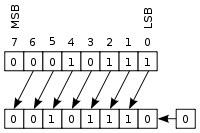
\includegraphics[scale=0.66]{bitfields/200px-Rotate_left_logically.png}
\caption{\IFRU{Как работает инструкция \SHL\protect\footnotemark}
{How \SHL instruction works\protect\footnotemark}}
\end{figure}

\footnotetext{\IFRU{иллюстрация взята из}{illustration taken from} wikipedia}

\IFRU{Макрос \TT{IS\_SET} на самом деле это операция логического И (\IT{AND}) 
и она возвращает ноль если бита там нет, 
либо эту же битовую маску, если бит там есть. 
В \CCpp, конструкция \TT{if()} срабатывает, если выражение внутри её не ноль, пусть хоть 123, 
поэтому все будет работать.}
{The \TT{IS\_SET} macro is in fact logical and operation (\IT{AND}) 
and it returns zero if specific bit is absent there,
or bit mask, if the bit is present.
\IT{if()} operator triggered in \CCpp if expression in it isn't zero, it might be even 123, that's why
it always working correctly.}

\IFRU{Компилируем}{Let's compile} (MSVC 2010):

\lstinputlisting{\IFRU{bitfields/14_1_ru.asm}{bitfields/14_1_en.asm}}

\IFRU{Вот так работает SHL (\IT{SHift Left})}{That's how SHL (\IT{SHift Left}) working}.

\IFRU{Скомпилируем то же и в}{Let's compile it in} GCC 4.4.1:

\lstinputlisting{bitfields/14_7_gcc.asm}

\IFRU{Инструкции сдвига также активно применяются при делении или умножении 
на числа-степени двойки (1, 2, 4, 8, итд).}
{Shift instructions are often used in division and multiplications by power of two numbers (1, 2, 4, 8, etc).}

\IFRU{Например:}{For example:}

\begin{lstlisting}
unsigned int f(unsigned int a)
{
	return a/4;
};
\end{lstlisting}

\IFRU{Имеем в итоге}{We got} (MSVC 2010):

\begin{lstlisting}
_a$ = 8							; size = 4
_f	PROC
	mov	eax, DWORD PTR _a$[esp-4]
	shr	eax, 2
	ret	0
_f	ENDP
\end{lstlisting}

\label{SHR}
\IFRU{Инструкция \SHR (\IT{SHift Right}) в данном примере сдвигает число на 2 бита вправо. 
При этом, освободившиеся два бита слева (т.е., самые 
старшие разряды), выставляются в нули. А самые младшие 2 бита выкидываются. 
Фактически, эти два выкинутых бита ~--- остаток от деления.}
{\SHR (\IT{SHift Right}) instruction in this example is shifting a number by 2 bits right.
Two freed bits at left (e.g., two most significant bits) are set to zero.
Two least significant bits are dropped.
In fact, these two dropped bits ~--- division operation remainder.}

\IFRU{Инструкция \SHR работает так же как и \SHL, только в другую сторону.}{\SHR instruction works just like as \SHL but in other direction.}

\begin{figure}[ht!]
\centering
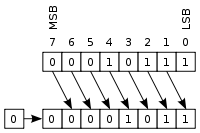
\includegraphics[scale=0.66]{bitfields/200px-Rotate_right_logically.png}
\caption{\IFRU{Как работает инструкция \SHR\protect\footnotemark}
{How \SHR instruction works\protect\footnotemark}}
\end{figure}

\footnotetext{\IFRU{иллюстрация взята из}{illustration taken from} wikipedia}

\IFRU{Для того, чтобы это проще понять, представьте себе десятичную систему счисления и число 23. 
23 можно разделить на 10 просто выкинув последний разряд (3 ~--- это остаток от деления). 
После этой операции останется 2 как частное
\footnote{результат деления}.}
{It can be easily understood if to imagine decimal numeral system and number 23.
23 can be easily divided by 10 just by dropping last digit (3 ~--- is division remainder). 
2 is leaving after operation as a quotient
\footnote{division result}.}

\IFRU{Так и с умножением. Умножить на 4 это просто сдвинуть число на 2 бита влево, 
вставив 2 нулевых бита справа (как два самых младших бита). 
Это как умножить 3 на 100 ~--- нужно просто дописать два нуля справа.}
{The same story about multiplication. Multiplication by 4 is just shifting the number to the left by 2 bits,
inserting 2 zero bits at right (as the last two bits).
It's just like to multiply 3 by 100 ~--- we need just to add two zeroes at the right.}

\subsection{\IFRU{Пример вычисления CRC32}{CRC32 calculation example}}

\newcommand{\URLCRCSRC}{\url{http://burtleburtle.net/bob/c/crc.c}}

\IFRU{Это распространенный табличный способ вычисления хеша алгоритмом 
CRC32\footnote{Исходник взят тут: \URLCRCSRC}.}
{This is very popular table-based CRC32 hash calculation 
method\footnote{Source code was taken here: \URLCRCSRC}.}

\lstinputlisting{bitfields/14_CRC.c}

\IFRU{Нас интересует функция \TT{crc()}. 
Кстати, обратите внимание, автор указал два инициализатора в выражении \TT{for()}: \TT{hash=len, i=0}. 
Стандарт \CCpp, конечно, допускает это. А в итоговом коде, вместо одной операции инициализации цикла, будет две.}
{We are interesting in \TT{crc()} function only.
By the way, please note: programmer used two loop initializers in \TT{for()} statement: \TT{hash=len, i=0}.
\CCpp standard allows this, of course. Emited code will contain two operations in loop initialization part
instead of usual one.}

\IFRU{Компилируем в MSVC с оптимизацией (\Ox). 
Для краткости, я приведу только функцию \TT{crc()}, с некоторыми комментариями.}
{Let's compile it in MSVC with optimization (\Ox).
For the sake of brevity, only \TT{crc()} function is listed here, with my comments.}

\lstinputlisting{\IFRU{bitfields/14_CRC_2_ru.asm}{bitfields/14_CRC_2_en.asm}}

\IFRU{Попробуем то же самое в GCC 4.4.1 с опцией \Othree:}
{Let's try the same in GCC 4.4.1 with \Othree option:}

\lstinputlisting{\IFRU{bitfields/14_CRC_gcc_O3_ru.asm}{bitfields/14_CRC_gcc_O3_en.asm}}

\IFRU{GCC немного выровнял начало тела цикла по 8-байтной границе, для этого добавил 
\NOP и \TT{lea esi, [esi+0]} (что тоже \IT{холостая операция}). 
Подробнее об этом смотрите в разделе о npad~\ref{sec:npad}.}
{GCC aligned loop start by 8-byte border by adding \NOP and \TT{lea esi, [esi+0]} (that's \IT{idle operation} too).
Read more about it in npad section~\ref{sec:npad}.}
